% 本模板根据中国科学院大学本科生公共必修课程《基础物理实验》Word模板格式编写
% 本模板由Shing-Ho Lin和Jun-Xiong Ji于2022年9月共同完成, 旨在方便LaTeX原教旨主义者和被Word迫害者写实验报告, 避免Word文档因插入过多图与公式造成卡顿. 
% 如有任何问题, 请联系: linchenghao21@mails.ucas.ac.cn
% This is the LaTeX template for experiment report of Experimental Physics courses, based on its provided Word template. 
% This template is completed by the joint collabration of Shing-Ho Lin and Junxiong Ji in September 2022. 
% Adding numerous pictures and equations leads to unsatisfying experience in Word. Therefore LaTeX is better. 
% Feel free to contact us via: linchenghao21@mails.ucas.ac.cn

\documentclass[11pt]{article}

\usepackage[a4paper]{geometry}
\geometry{left=2.0cm,right=2.0cm,top=2.5cm,bottom=2.5cm}

\usepackage{ctex} % 支持中文的LaTeX宏包
\usepackage{amsmath,amsfonts,graphicx,subfigure,amssymb,bm,amsthm,mathrsfs,mathtools,breqn} % 数学公式和符号的宏包集合
\usepackage{algorithm,algorithmicx} % 算法和伪代码的宏包
\usepackage[noend]{algpseudocode} % 算法和伪代码的宏包
\usepackage{fancyhdr} % 自定义页眉页脚的宏包
\usepackage[framemethod=TikZ]{mdframed} % 创建带边框的框架的宏包
\usepackage{fontspec} % 字体设置的宏包
\usepackage{adjustbox} % 调整盒子大小的宏包
\usepackage{fontsize} % 设置字体大小的宏包
\usepackage{tikz,xcolor} % 绘制图形和使用颜色的宏包
\usepackage{multicol} % 多栏排版的宏包
\usepackage{multirow} % 表格中合并单元格的宏包
\usepackage{pdfpages} % 插入PDF文件的宏包
\RequirePackage{listings} % 在文档中插入源代码的宏包
\RequirePackage{xcolor} % 定义和使用颜色的宏包
\usepackage{wrapfig} % 文字绕排图片的宏包
\usepackage{bigstrut,multirow,rotating} % 支持在表格中使用特殊命令的宏包
\usepackage{booktabs} % 创建美观的表格的宏包
\usepackage{circuitikz} % 绘制电路图的宏包

\definecolor{dkgreen}{rgb}{0,0.6,0}
\definecolor{gray}{rgb}{0.5,0.5,0.5}
\definecolor{mauve}{rgb}{0.58,0,0.82}
\lstset{
  frame=tb,
  aboveskip=3mm,
  belowskip=3mm,
  showstringspaces=false,
  columns=flexible,
  framerule=1pt,
  rulecolor=\color{gray!35},
  backgroundcolor=\color{gray!5},
  basicstyle={\small\ttfamily},
  numbers=none,
  numberstyle=\tiny\color{gray},
  keywordstyle=\color{blue},
  commentstyle=\color{dkgreen},
  stringstyle=\color{mauve},
  breaklines=true,
  breakatwhitespace=true,
  tabsize=3,
}

% 轻松引用, 可以用\cref{}指令直接引用, 自动加前缀. 
% 例: 图片label为fig:1
% \cref{fig:1} => Figure.1
% \ref{fig:1}  => 1
\usepackage[capitalize]{cleveref}
% \crefname{section}{Sec.}{Secs.}
\Crefname{section}{Section}{Sections}
\Crefname{table}{Table}{Tables}
\crefname{table}{Table.}{Tabs.}

\setmainfont{Palatino Linotype.ttf}
\setCJKmainfont{SimHei.ttf}
% \setCJKsansfont{Songti.ttf}
% \setCJKmonofont{SimSun.ttf}
\punctstyle{kaiming}
% 偏好的几个字体, 可以根据需要自行加入字体ttf文件并调用

\renewcommand{\emph}[1]{\begin{kaishu}#1\end{kaishu}}

%改这里可以修改实验报告表头的信息
\newcommand{\experiName}{温度的测量,用动态法测定良导体的热导率}
\newcommand{\supervisor}{赵同宪}
\newcommand{\name}{张欣培}
\newcommand{\studentNum}{2022K8009922001}
\newcommand{\class}{01}
\newcommand{\group}{10}
\newcommand{\seat}{11}
\newcommand{\dateYear}{2023}
\newcommand{\dateMonth}{10}
\newcommand{\dateDay}{16}
\newcommand{\room}{教427}
\newcommand{\others}{$\square$}
%% 如果是调课、补课, 改为: $\square$\hspace{-1em}$\surd$
%% 否则, 请用: $\square$
%%%%%%%%%%%%%%%%%%%%%%%%%%%

\begin{document}

%若需在页眉部分加入内容, 可以在这里输入
% \pagestyle{fancy}
% \lhead{\kaishu 测试}
% \chead{}
% \rhead{}

\begin{center}
    \LARGE \bf 《\, 基\, 础\, 物\, 理\, 实\, 验\, 》\, 实\, 验\, 报\, 告
\end{center}

\begin{center}
    \noindent \emph{实验名称}\underline{\makebox[25em][c]{\experiName}}
    \emph{指导教师}\underline{\makebox[8em][c]{\supervisor}}\\
    \emph{姓名}\underline{\makebox[6em][c]{\name}} 
    % 如果名字比较长, 可以修改box的长度"6em"
    \emph{学号}\underline{\makebox[10em][c]{\studentNum}}
    \emph{分班分组及座号} \underline{\makebox[5em][c]{\class \ -\ \group \ -\ \seat }\emph{号}} (\emph{例}:\, 1\,-\,04\,-\,5\emph{号})\\
    \emph{实验日期} \underline{\makebox[3em][c]{\dateYear}}\emph{年}
    \underline{\makebox[2em][c]{\dateMonth}}\emph{月}
    \underline{\makebox[2em][c]{\dateDay}}\emph{日}
    \emph{实验地点}\underline{{\makebox[4em][c]\room}}
    \emph{调课/补课} \underline{\makebox[3em][c]{\others\ 是}}
    \emph{成绩评定} \underline{\hspace{5em}}
    {\noindent}
    \rule[8pt]{17cm}{0.2em}
\end{center}

%\tableofcontents

\begin{center}
    \Large \bf 第一部分\qquad 动态法测定良导体的热导率
\end{center}

\section{实验目的}

\begin{enumerate}
    \item 了解热波的概念。
    \item 了解静态法和动态法测热导率的优劣。
\end{enumerate}

\section{实验仪器}

    \hspace*{2em} 绝热材料包裹的热导体(铜,铝)及测温、加热,冷却装置,计算机等。

\section{实验原理}
\begin{enumerate}
    \item 程序控制加热端以方波的形式输出热,另一端持续输入冷却水降温。体现在整个热导体上是正弦型热波温度传导。测温器以2cm间距间隔排列,连续测量温度,生成多点温度曲线,能够体现热波的传导过程。通过计算温度峰值的时间间距,计算平均值,可以得到和热传导相关的量。
    \newline 冷却水不仅在非加热段冷却,还起到冷却热源的作用,要持续通入常温水,防止电路元件过热,保持温度动态平衡。关闭设备时,应最后关闭冷却水。
    \item 处理数据时,直接对曲线处理较为困难。肉眼寻找每段曲线极大值/极小值后取最早的时间/平均的时间较为方便。取平均时间,数据偏差较小,采用此方法。
\end{enumerate}

\section{实验步骤与实验数据}

\begin{enumerate}
    \item 记录数据
    \begin{enumerate}
        \item 打开冷却水,打开电脑,打开一体化仪器开关。
        \item 打开控制程序,选择铜样本,开始测量,静置一段时间。前期可能出现突变数据和不稳定数据,应在数据处理时摒弃。
        \item 保存铜样本数据,选择铝样本,开始测量,静置一段时间。
        \item 保存铝样本数据,关闭设备,关闭冷却水。
    \end{enumerate}
    \item 数据处理
    \begin{enumerate}
        \item 将数据格式转换成表格形式。
        \item 取中后段数据,取每个测温点最先到温度极大值的时间并记录,记录6个点。
        \item 计算5段的热传导速度,取平均值,记为V。
        \item 由公式
        \[
            k=\frac{V^{2}C\rho }{4\pi f}=\frac{V^{2}C\rho }{4\pi }T
        \]
        计算热导率k。其中,$V$为测量量热传导速度,$D$为热扩散系数,$C$为比热容,$\rho$为密度,$f$为频率,$T$为周期。
        \newline 样品比热数据——铜:$0.385J/gK$;铝: $0.9J/gK$。样品密度数据——铜: $8.92g/cm^{3}$; 铝: $2.7g/cm^{3}$。
        
    \end{enumerate}
    \item 数据记录如下。注:此处使用的数据和课上填写的不为同一数据,但仍旧为课上实验所得的数据。  
    % Table generated by Excel2LaTeX from sheet 'Sheet1'
        \begin{table}[H]
            \centering
            \caption{动态法测铜的热导率}
            \begin{center}
                \begin{tabular}{|l|r|r|r|r|r|r|}\hline 
                    测量点n  & 1     & 2     & 3     & 4     & 5     & 6 \\\hline
                    对应峰值时间t($s$) & 3518.28 & 3523.52 & 3529.28 & 3536.78 & 3545.78 & 3552.78 \\\hline
                    波速($m/s$) & 0.0038 & 0.0035 & 0.0027 & 0.0022 & 0.0029 &  \\\hline
                \end{tabular}%
                
            \end{center}
            波速平均值:$0.0029m/s$,\qquad 热导率:$413.7W/(m\cdot K)$
            
          %\label{tab:addlabel}%
        \end{table}%

                % Table generated by Excel2LaTeX from sheet 'Sheet1'
        \begin{table}[H]
          \centering
          \caption{动态法测铝的热导率}
            \begin{center}
                \begin{tabular}{|l|r|r|r|r|r|r|}\hline
                    测量点n  & 1     & 2     & 3     & 4     & 5     & 6 \\\hline
                    对应峰值时间t(s) & 2259.28 & 2264.28 & 2272.04 & 2281.04 & 2292.52 & 2299.78 \\\hline
                    波速(m/s) & 0.0040  & 0.0026  & 0.0022  & 0.0017  & 0.0028  &  \\\hline
                \end{tabular}%
            \end{center}
            波速平均值:$0.0027m/s$,\qquad 热导率:$253.7W/(m\cdot K)$
          %\label{tab:addlabel}%
        \end{table}%


\end{enumerate}

\section{实验结论、反思、收获与总结}
\begin{enumerate}
    \item 要获得T-x曲线,叠加同一时间不同测温点的温度即可。
    \item T-t曲线振幅越来越小,因为后面的测温点距离热源越来越远,相对于热源的热传导越来越慢。振幅小会导致峰值持续时间长,会增大实验误差。
    \item 铜棒比铝棒测温点多,因为铝热导率是铜的两倍以上,距离热源远的测温点会振幅小,峰值时间长,效果较差,误差更大。因此测温点可以减少。
    \item 实验误差来源:
    \newline (1)测温点测温为一小块区域,不为精确的点,提升测温误差。
    \newline (2)测温器在使用前未统一校准,多次使用后会有仪器误差。
    \newline (3)测温点精度不够高,使峰值时间持续较长,影响测量。
    \newline (4)实际上,测温点不是同时测温,而是走马灯式连续测温。这会带来测温时间的微小误差,第一个点到最后一个点的测量时间恰为一个测量时间周期。本误差周期性稳定,只会微小影响到热导速度。实际计算时,此部分误差小于计算误差。
    \newline (5)本仪器一体化,内部状态无法确定,可能存在如导热材料不均匀等未知误差。
    \newline (6)如果测温点距离更大,测量会更精确,但会提升仪器成本。作为演示仪器,无需增大测温点距离。
    \item 热波是热传导距离不同导致每点的温度变化速度不同。热波由方波生成正弦型波。热波传导速度与热导率有关,热导率越大,热波传导速度越快。
    \item 静态法测热导率需要恒温条件,实验要求严苛。动态法不太关心外部条件,只需要保证输入热源波的周期性稳定即可,条件简单。静态法测量热流,动态法把热流的测量转化为长度的测量,易于操作。
    
\end{enumerate}

%\tableofcontents

\begin{center}
    \vspace*{1em}
    \Large \bf 第二部分\qquad 温度的测量和温度计的设计
\end{center}
\setcounter{section}{0}
\section{实验目的}
\begin{enumerate}
    \item 了解电位差计测热电动势的方法。
    \item 学习使用平衡电桥,用平衡电桥测量并绘制热敏电阻和铜电阻的温度特性曲线。
    \item 根据热敏电阻相关参数,设计非平衡电桥实现对热敏电阻的实时测量。
\end{enumerate}

\section{实验仪器}
\hspace*{2em} 热电偶温度计,铜电阻温度计,热敏电阻温度计,测温仪,控温炉,多功能电桥,电位差计,导线,冰水混合物等。

\section{实验原理}
\begin{enumerate}
    \item 电位差计测电压:电位差计根据被测电压和已知电压相互补偿 (即平衡)的原理制成。此时电路中无电流,无电池内阻产生的电压降,更精准。本次实验使用的电位差计最小刻度0.05$mV$,且有倍数,能够测量$10^{-5}$精度的电压。
    \item 平衡电桥测电阻:电桥测电阻的原理是根据电桥平衡条件,即$R_{1}R_{4}=R_{2}R_{3}$,测量未知电阻。平衡电桥平衡条件是:两条支路中间的导线两端电势差为0,实际测量时可精确到$mV$测量,精度很高。
    \item 热电偶温度计直接测量温度,并把温度信号转换成热电动势信号,通过电气仪表(二次仪表)转换成被测介质的温度。其精度高,测量范围广。
    \item 热敏电阻是一种电阻值随温度变化明显的电阻,随温度变化的趋势各不相同。其特性也可以将温度信号转化为电信号,但是精度较低。
\end{enumerate}

\section{实验步骤与实验数据}
\subsection{平衡电桥测电阻和电位差计测电压}
\begin{enumerate}
    \item 连接设备线路,开启电源。
    \item 电位差计调零。热电偶低温端插入冰水混合物。
    \item 连接线路,用平衡电桥测量室温下热敏电阻和铜电阻值并记录,用电位差计测量室温下热电偶的温差电动势并记录。
    \item 提升温控仪温度升温,待温度稳定后,用平衡电桥测量热敏电阻和铜电阻值并记录,用电位差计测量热电偶的温差电动势并记录。
    \item 重复第四步,测量多组数据并记录,测温范围在30-50$^{\circ}C$。
    \item 关闭设备,清理实验台。
    \newline 实验数据记录如下:
    % Table generated by Excel2LaTeX from sheet 'Sheet1'
   \begin{table}[H]
     \centering
     \caption{电位差计测热电偶温差电动势}
     室温:$t=30.7^{\circ}C$ \qquad 电动势:$E_{x}=1.06mV$ \qquad 冷端温度:$t_{0}=0^{\circ}C$
       \begin{center}
           \begin{tabular}{|l|r|r|r|r|r|}\hline
               温度$t(^{\circ}C)$ & 30.7  & 35.7  & 40.0  & 45.3  & 50.0  \\\hline
               电动势$E_{x}(mV)$ & 1.06  & 1.30  & 1.47  & 1.68  & 1.87  \\\hline
           \end{tabular}%
       \end{center}
       温差电系数$\alpha = 0.0415mV/^{\circ}C$
     %\label{tab:addlabel}%
   \end{table}%
    % Table generated by Excel2LaTeX from sheet 'Sheet1'
        \begin{table}[H]
          \centering
          \caption{平衡电桥测铜电阻温度特性曲线}
          室温:$t=30.7^{\circ}C$ \qquad 电阻:$R_{x}=58.8\Omega$
            \begin{center}
                \begin{tabular}{|l|r|r|r|r|r|}\hline
                    温度$t(^{\circ}C)$ & 30.7  & 35.8  & 39.4  & 45    & 50.2 \\\hline
                    电阻$R_{x}(\Omega)$ & 58.8  & 59.9  & 60.7  & 61.9  & 63 \\\hline
                \end{tabular}%
            \end{center}
            电阻温度系数$\alpha = 0.2157\varOmega/^{\circ}C$
          %\label{tab:addlabel}%
        \end{table}%
        \begin{figure}[H]
            \centering
            \begin{minipage}[t]{0.49\linewidth}
                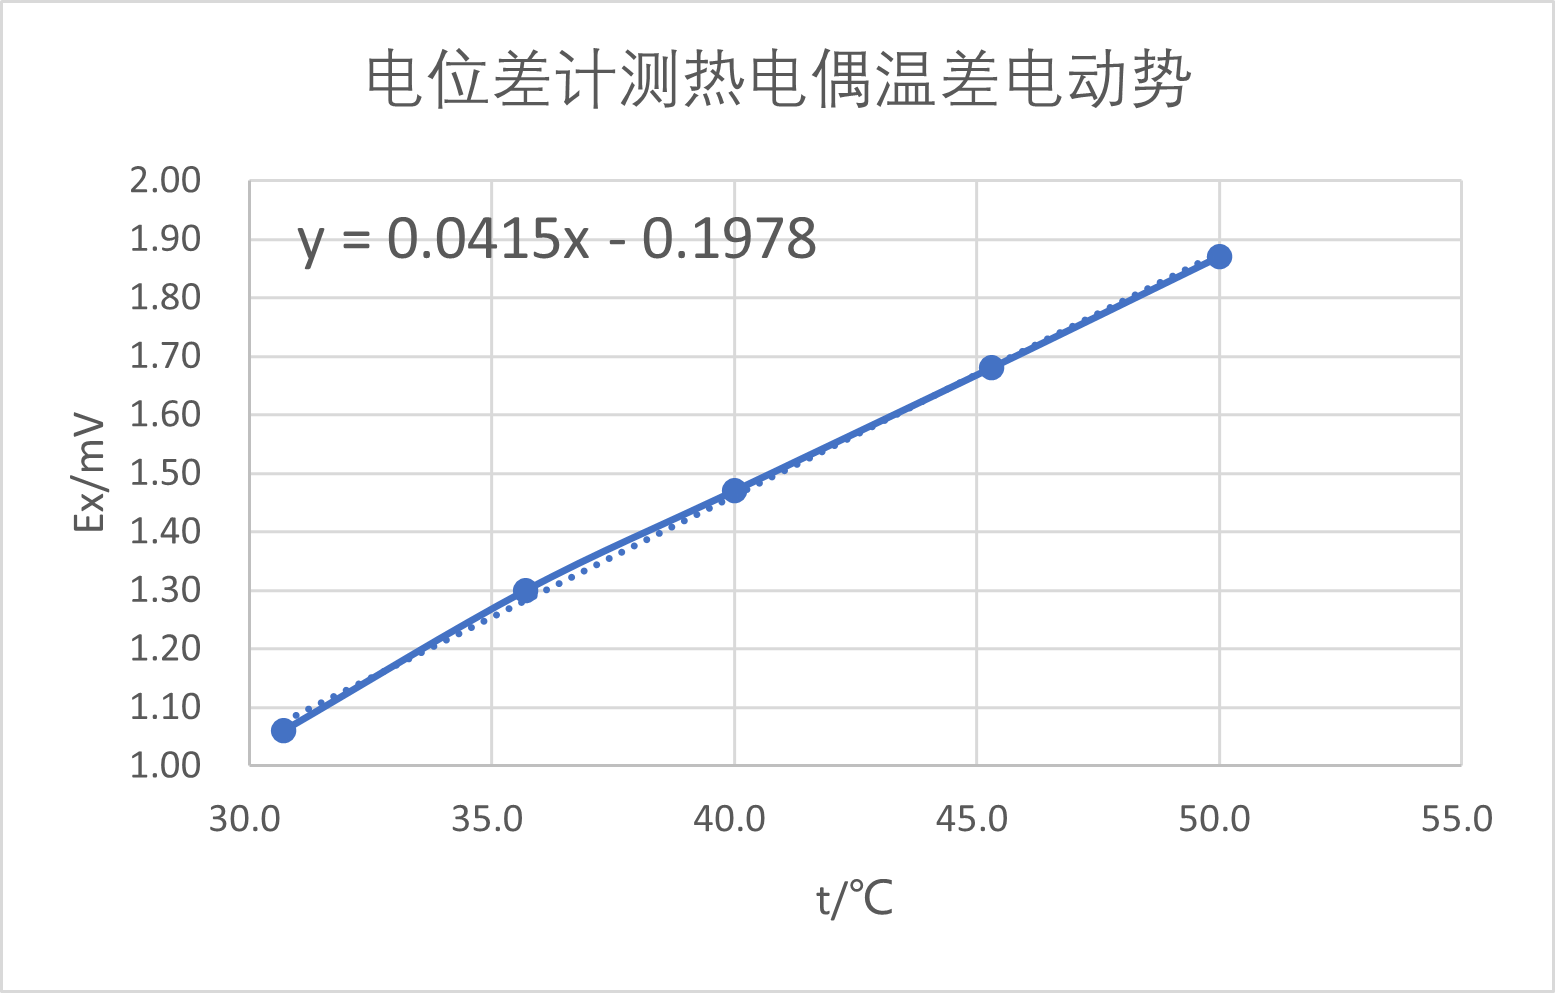
\includegraphics[width=8cm]{Fig/1.png}
                \caption{热电偶温差电动势}
            \end{minipage}
            \begin{minipage}[t]{0.49\linewidth}
                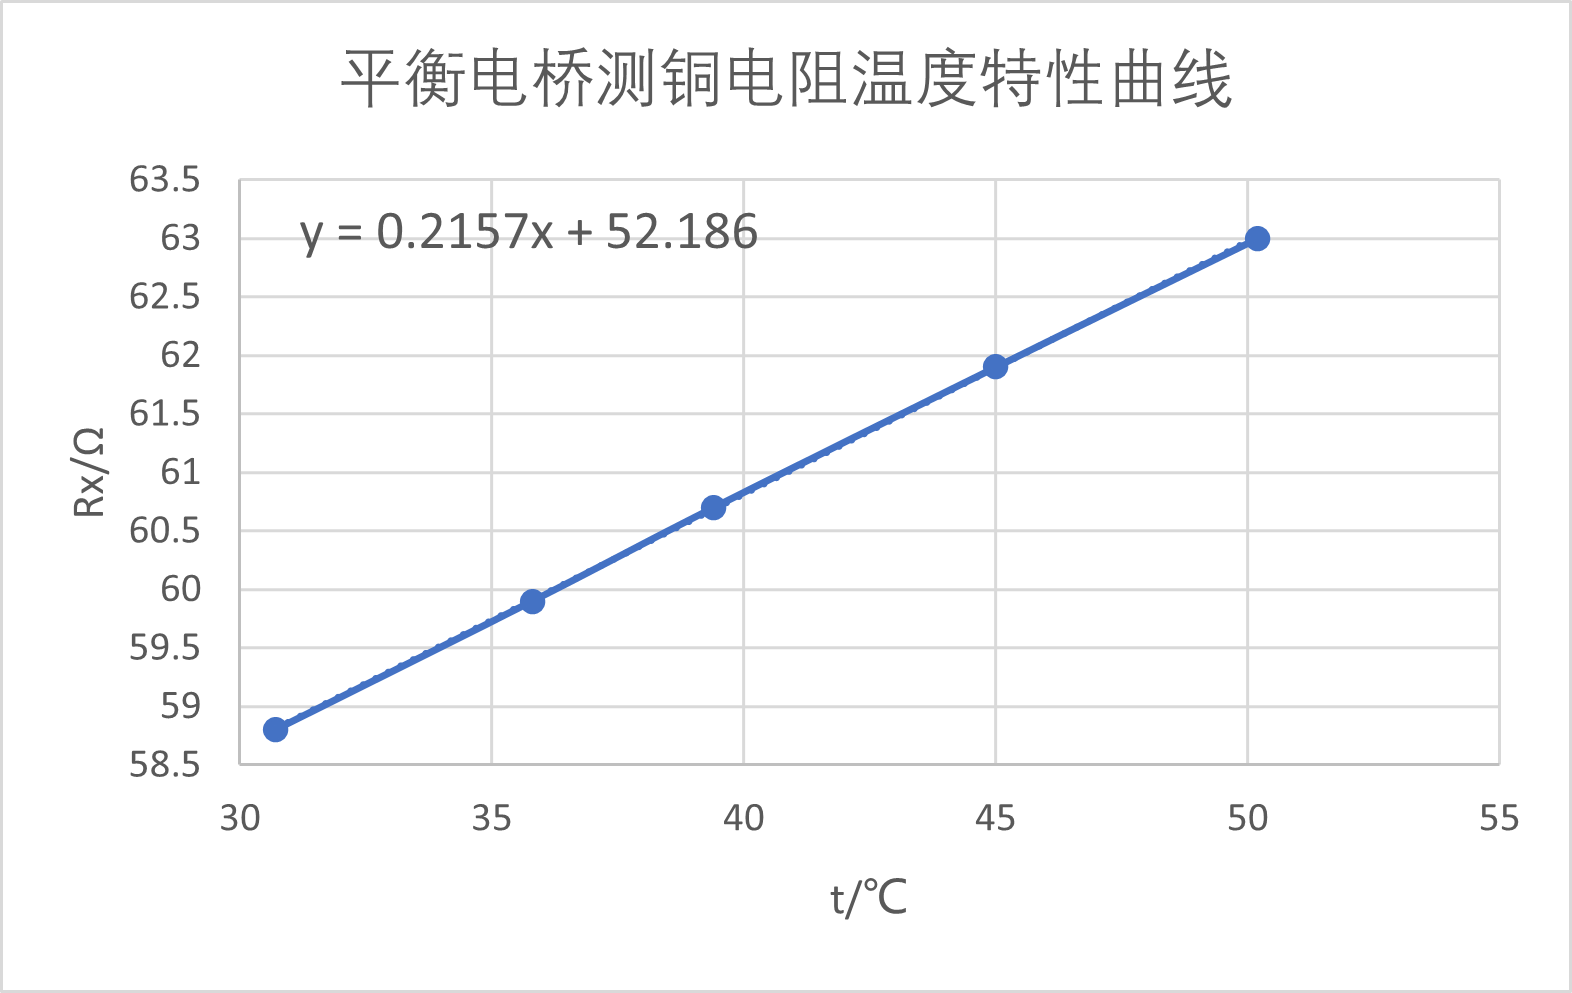
\includegraphics[width=8cm]{Fig/2.png}
                \caption{铜电阻温度特性曲线}
            \end{minipage}
            
            
        \end{figure}
        % Table generated by Excel2LaTeX from sheet 'Sheet1'
        \begin{table}[H]
          \centering
          \caption{热敏电阻温度特性曲线}
          室温:$t=30.7^{\circ}C$ \quad 电阻:$R_{x}=$(未测量)$\Omega$。(注:开始时忘记测量本组数据,后期降温速度过慢,来不及补充数据)
            \begin{center}
                \begin{tabular}{|l|r|r|r|r|r|r|r|}\hline
                    $t(^{\circ}C)$   & 40.0    & 42.2  & 42.9  & 44.2  & 47.0    & 49.0    & 51.0 \\\hline
                    $R_{t}(\Omega)$   & 1552.2 & 1408  & 1368  & 1297  & 1165  & 1066  & 986 \\\hline
                    $T(K)$     & 313.15 & 315.35 & 316.05 & 317.35 & 320.15 & 322.15 & 324.15 \\\hline
                    $\ln R_{t}$  & 7.347429 & 7.249926 & 7.221105 & 7.167809 & 7.060476 & 6.971669 & 6.893656 \\\hline
                    $1/T$   & 0.003193 & 0.003171 & 0.003164 & 0.003151 & 0.003124 & 0.003104 & 0.003085 \\\hline
                \end{tabular}%
            \end{center}
          %\label{tab:addlabel}%
        \end{table}%
        \begin{figure}[H]
            \centering
            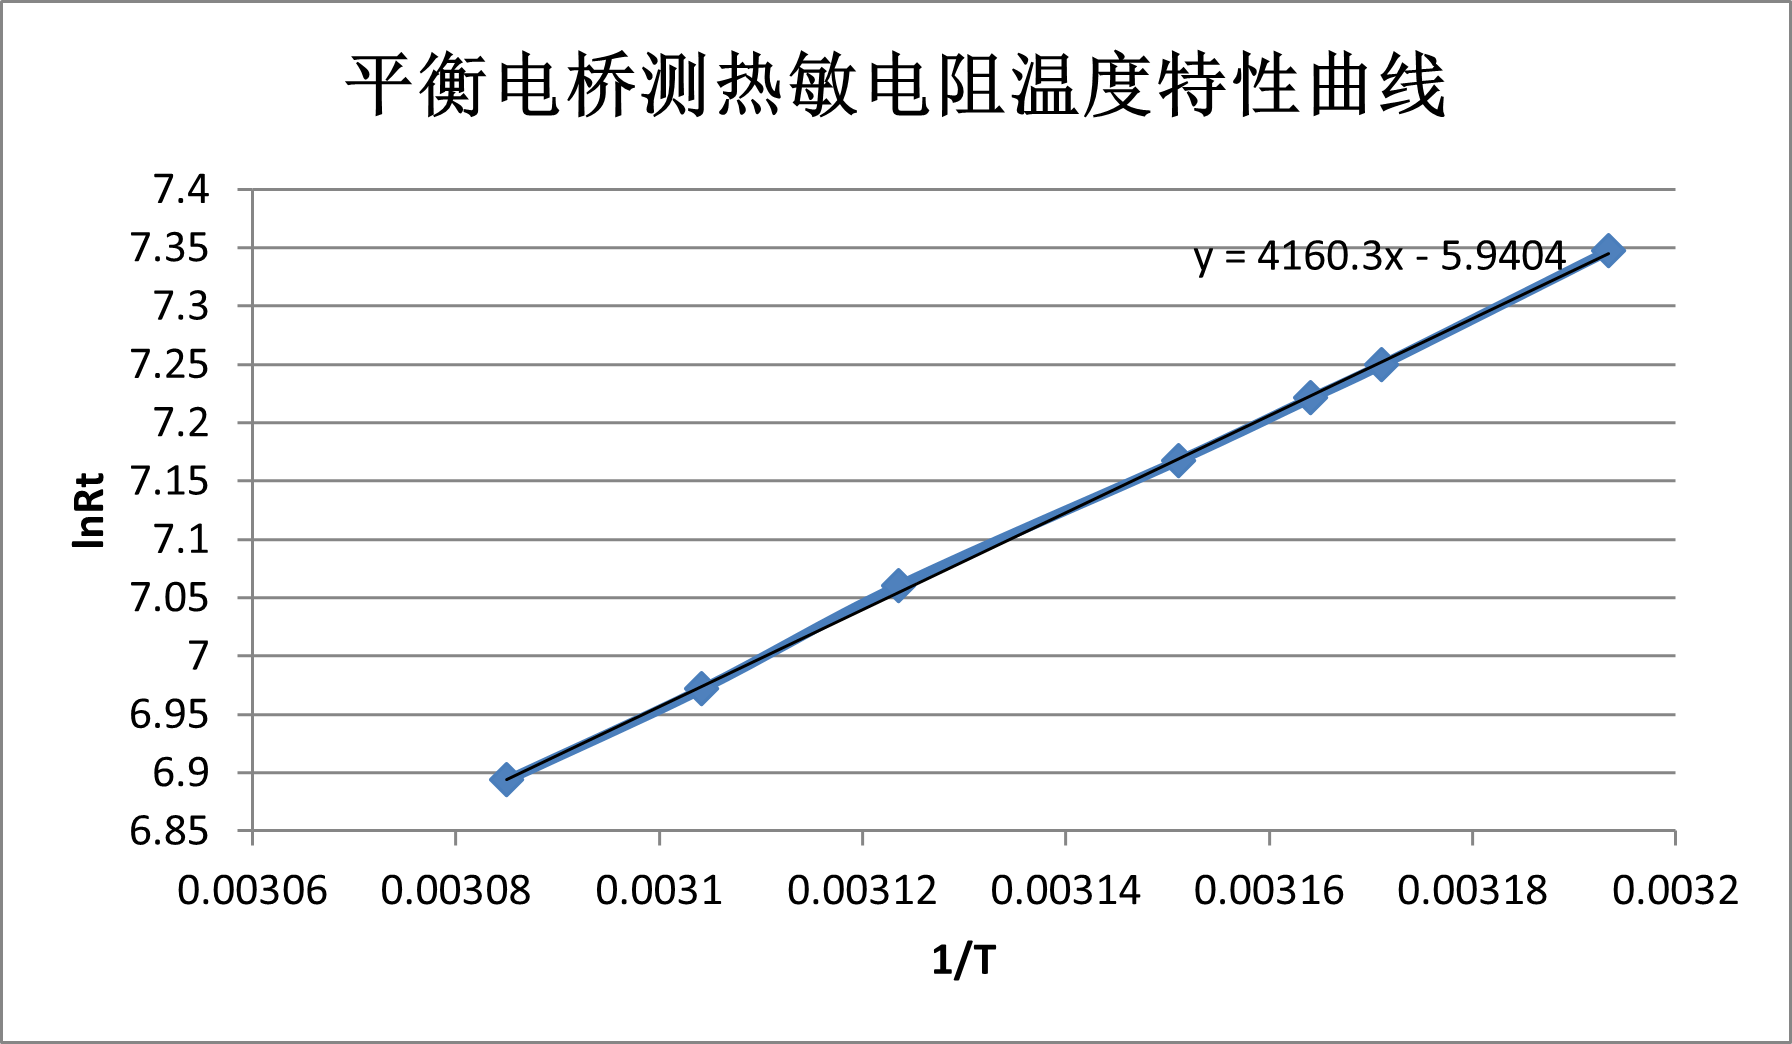
\includegraphics[width=10cm]{Fig/3.png}
            \caption{热敏电阻温度特性曲线}
        \end{figure}
        由热敏电阻的电阻温度特性函数$R_{t}=Ae^{\frac{B}{T}}$,即$\ln R_{t}=\ln A+\frac{B}{T}$,由图3拟合数据得热敏温度特性常数$A=0.02632$ \qquad $B=4160$
   
\end{enumerate}
    

\subsection{设计非平衡电桥测温器}
\begin{enumerate}
    \item 连接设备线路,开启电源。
    \item 根据热敏电阻温度特性曲线计算出的热敏温度特性常数$A$和$B$,计算工作电源电压,$R_{1}$,$R_{2}$,$R_{3}$阻值,设计非平衡电桥测温器。
    \newline 具体表达式为:\quad
    \[ 
    E=\frac{4BT_{1}^{2}}{4T_{1}^{2}-B_{2}} m 
    \qquad R_{2}=\frac{B-2T}{B+2T} R_{xT_{1}}
    \qquad  \frac{R_{1}}{R_{3}} = \frac{2BE}{(B+2T_{1}) E-2B\lambda} -1
    \]
    其中,$m$是灵敏度,$\lambda$表示温度区间中间值(比如上面的$40^{\circ}C$)时,对应的$U_{0}$值。
    \item 依照设计调整平衡电桥。微调$R_{2}$,使$t_{1}=40.0^{\circ}C$时电桥电压读数恰为$-400mV$。
    \item 逐渐提升设定温度$t$,读取测试电压$U_{0}$。
    \item 重复第三步,测量多组数据并记录,测温范围在30-50$^{\circ}C$。
    \item 计算测试温度:\quad $t'=\frac{U_{0}-\lambda}{m}+t_{1}$。
    \item 关闭设备,清理实验台。
    \newline 相关数据如下:
    \newline 温度区间:$30-50^{\circ}C$ \qquad 
    \newline 热敏电阻特性常数:$A=0.02632$ ,\quad $B=4160$; \qquad 
    \newline 表头参数选择:$\lambda = -0.4V$,\quad $m=-0.01V/^{\circ}C$;\qquad 
    \newline 工作电源电压:$E=0.96V$,\quad $R_{1}=1146\Omega$,\quad $\frac{R_{1}}{R_{3}}=0.00816$;\qquad 
    \newline 实际值:$R_{2}=1011\Omega$,\quad $R_{1}=8.2\Omega$,\quad $R_{3}=1000\Omega$。
    % Table generated by Excel2LaTeX from sheet 'Sheet1'
        \begin{table}[H]
          \centering
          \caption{非平衡电桥热敏电阻温度计的设计}
            \begin{center}
                \begin{tabular}{|l|r|r|r|r|r|}\hline
                    设定温度$t(^{\circ}C)$ & 40.0  & 42.5  & 45.5  & 48.1  & 49.3  \\\hline
                    测试电压$U_{0}(mV)$ & -400  & -424  & -452  & -478  & -487 \\\hline
                    测试温度$t'(^{\circ}C)$ & 40.0  & 42.4  & 45.2  & 47.8  & 48.7  \\\hline
                \end{tabular}%
            \end{center}
            注:$t_{1}=40^{\circ}C$。
          %\label{tab:addlabel}%
        \end{table}%

\end{enumerate}
\section{实验结论、反思、收获与总结}
    \begin{enumerate}
        \item 加热炉降温速度很慢,升温较快。实验中尽量不要前期漏掉数据,以免浪费时间。
        \item 我实际实验时热敏电阻连接错误,导致第一版热敏电阻数据测量错误,为节约时间使用了其他座位的加热炉。第二版数据区间大致是$40^{\circ}C-50^{\circ}C$,温度区间较小,会增大图像拟合误差。这使得我计算出的热敏温度特性常数误差增大,导致非平衡电桥温度计误差增大。
        \item 读数时要等待温度稳定后再读数。读电阻时无需读取有效数字超过三位,读数太精确会让实验更复杂。
        \item 相信自己的实验数据,在和其他同学相差小于一个数量级即为正确,尽管有误差,但是最后数据精准度足够。
        \item 四线制可完全消除引线的电阻影响,主要用于高精度的温度检测。低温下四线式伏安法精度更高。非平衡电阻测温法可做到电路电压/电流趋于零,也能克服引线电阻,其测量范围更广,且更方便。
        \item 工业仪表中使用的三线式非平衡电桥测温度消除引线电阻:保持引线规格一致,即长度、截面积、材质一致,降低引线差异。
    \end{enumerate}
    
    \newpage
    \begin{center}
        \Large \bf 第三部分\qquad 实验原始记录
    \end{center}
    \begin{figure}[H]
        \centering
        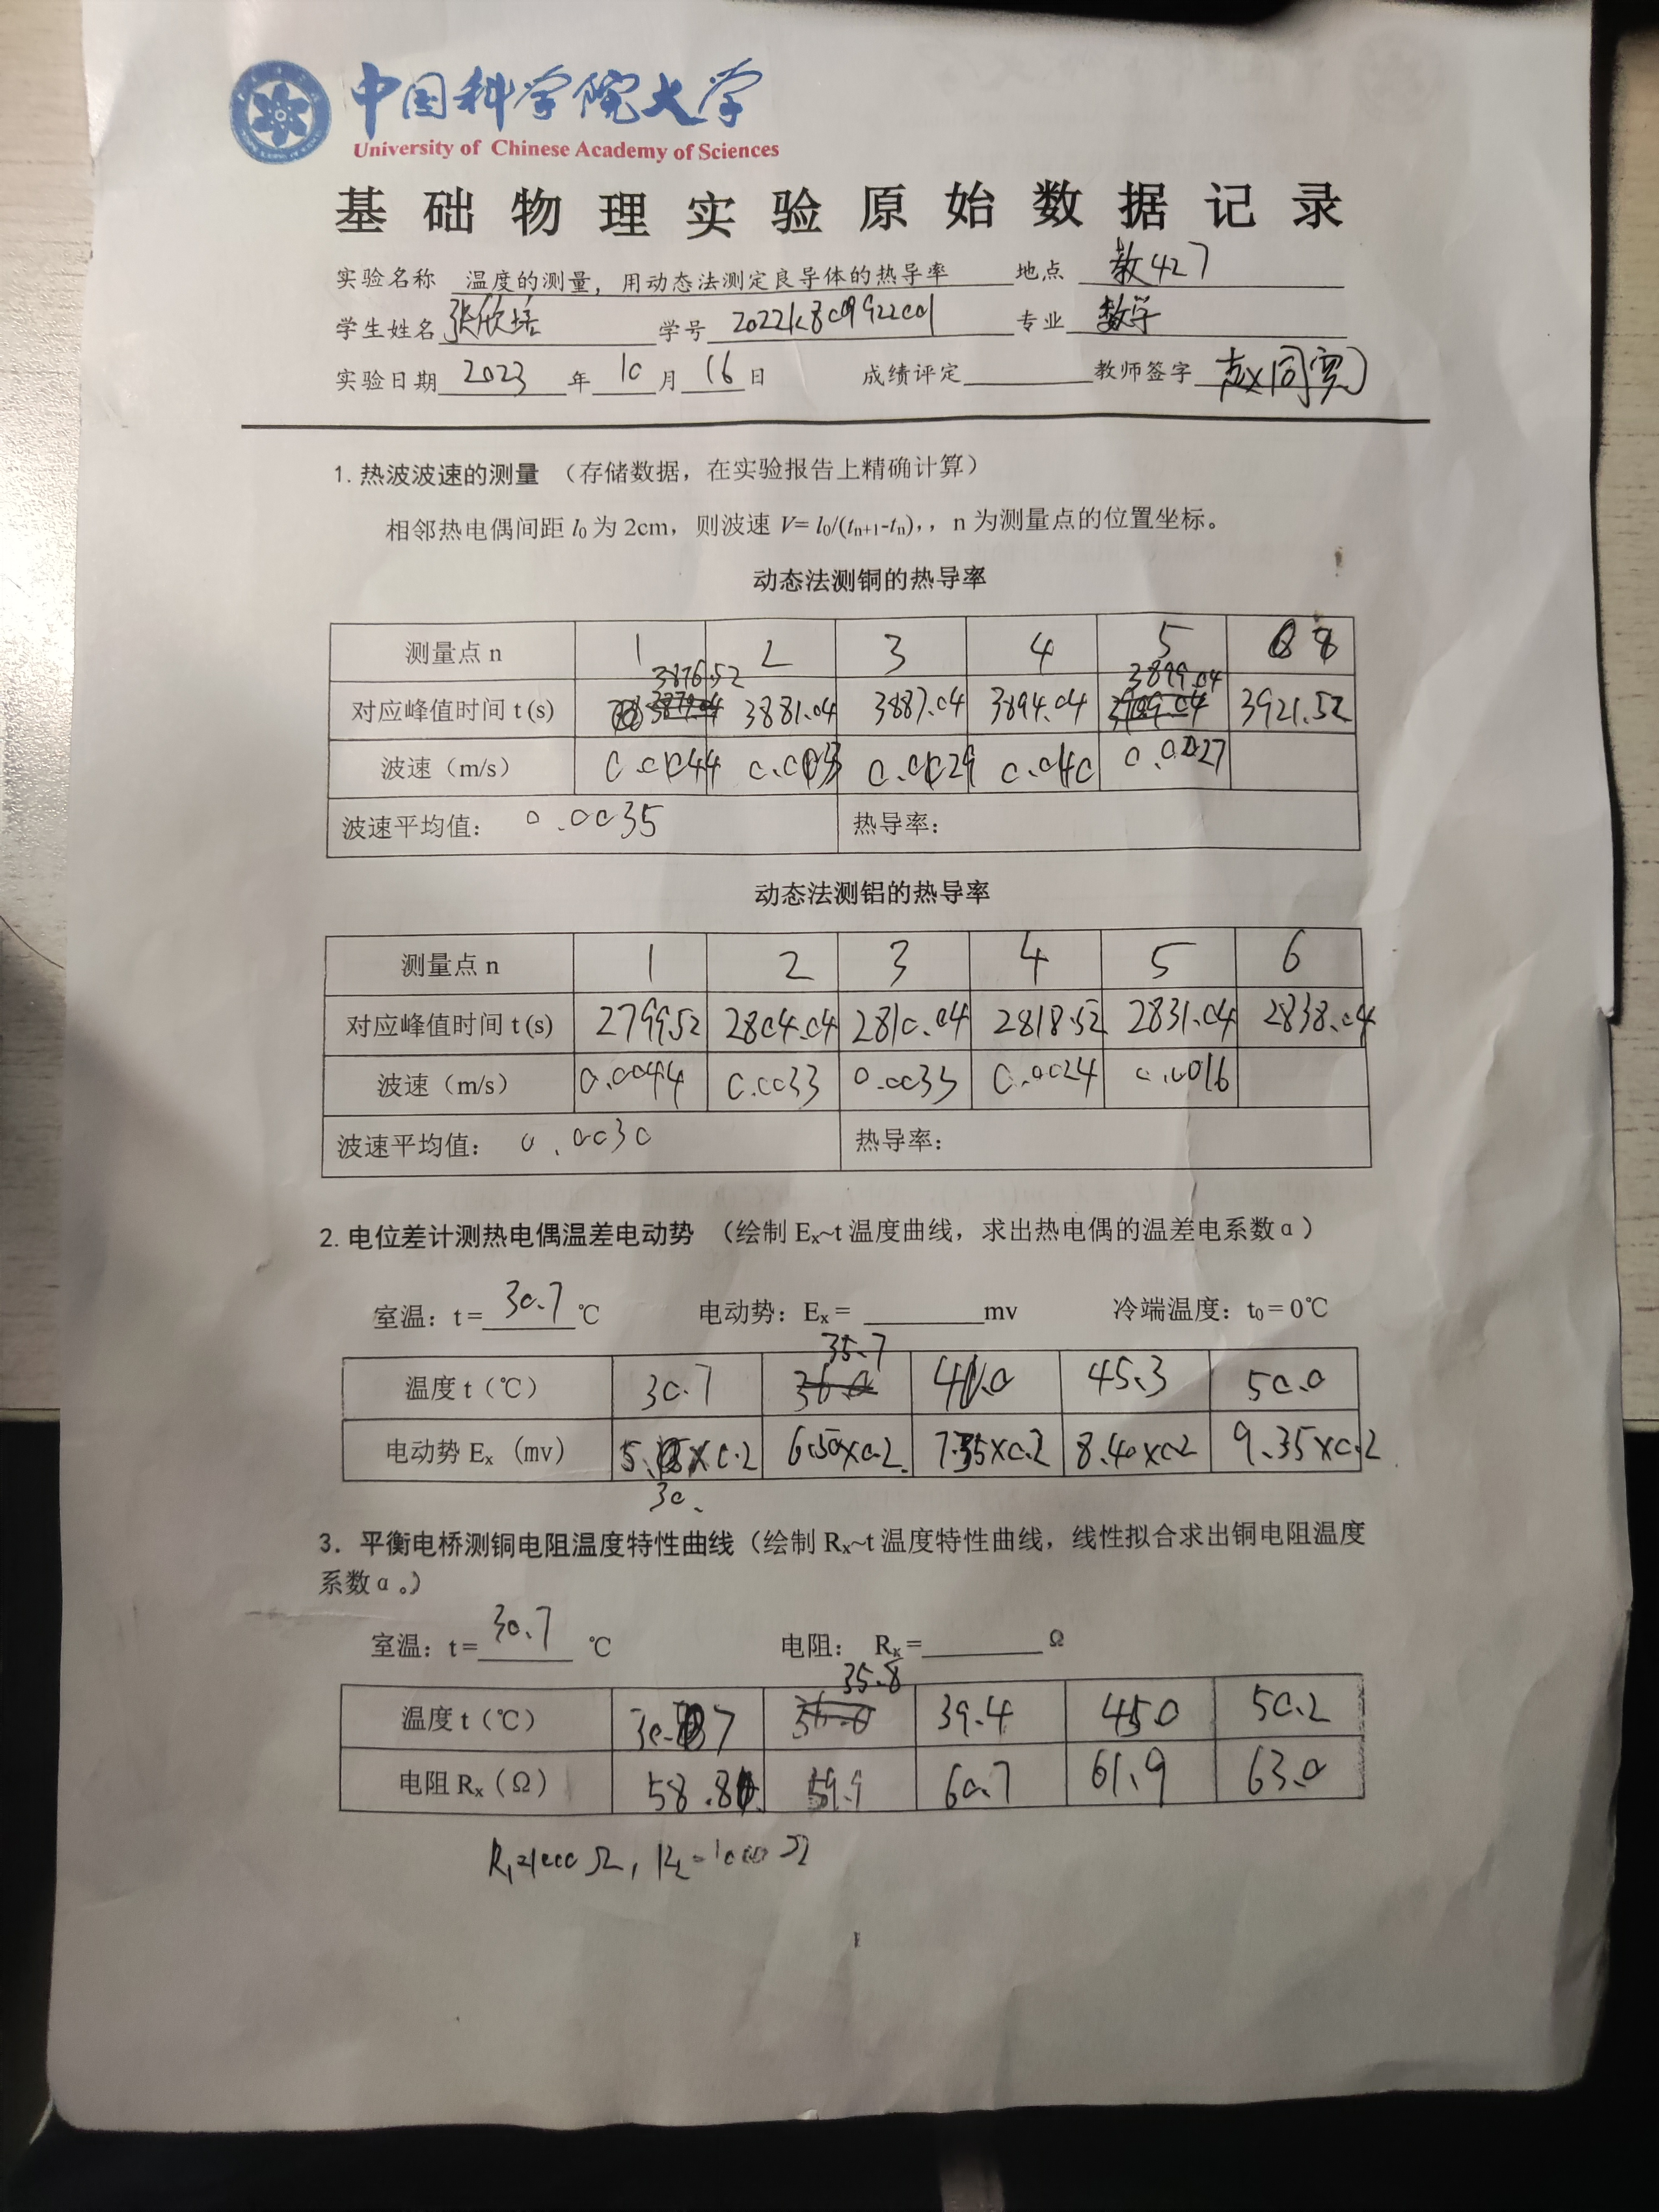
\includegraphics[width=15cm]{Fig/4.jpg}
        \caption{实验原始记录1}
    \end{figure}
    \begin{figure}[H]
        \centering
        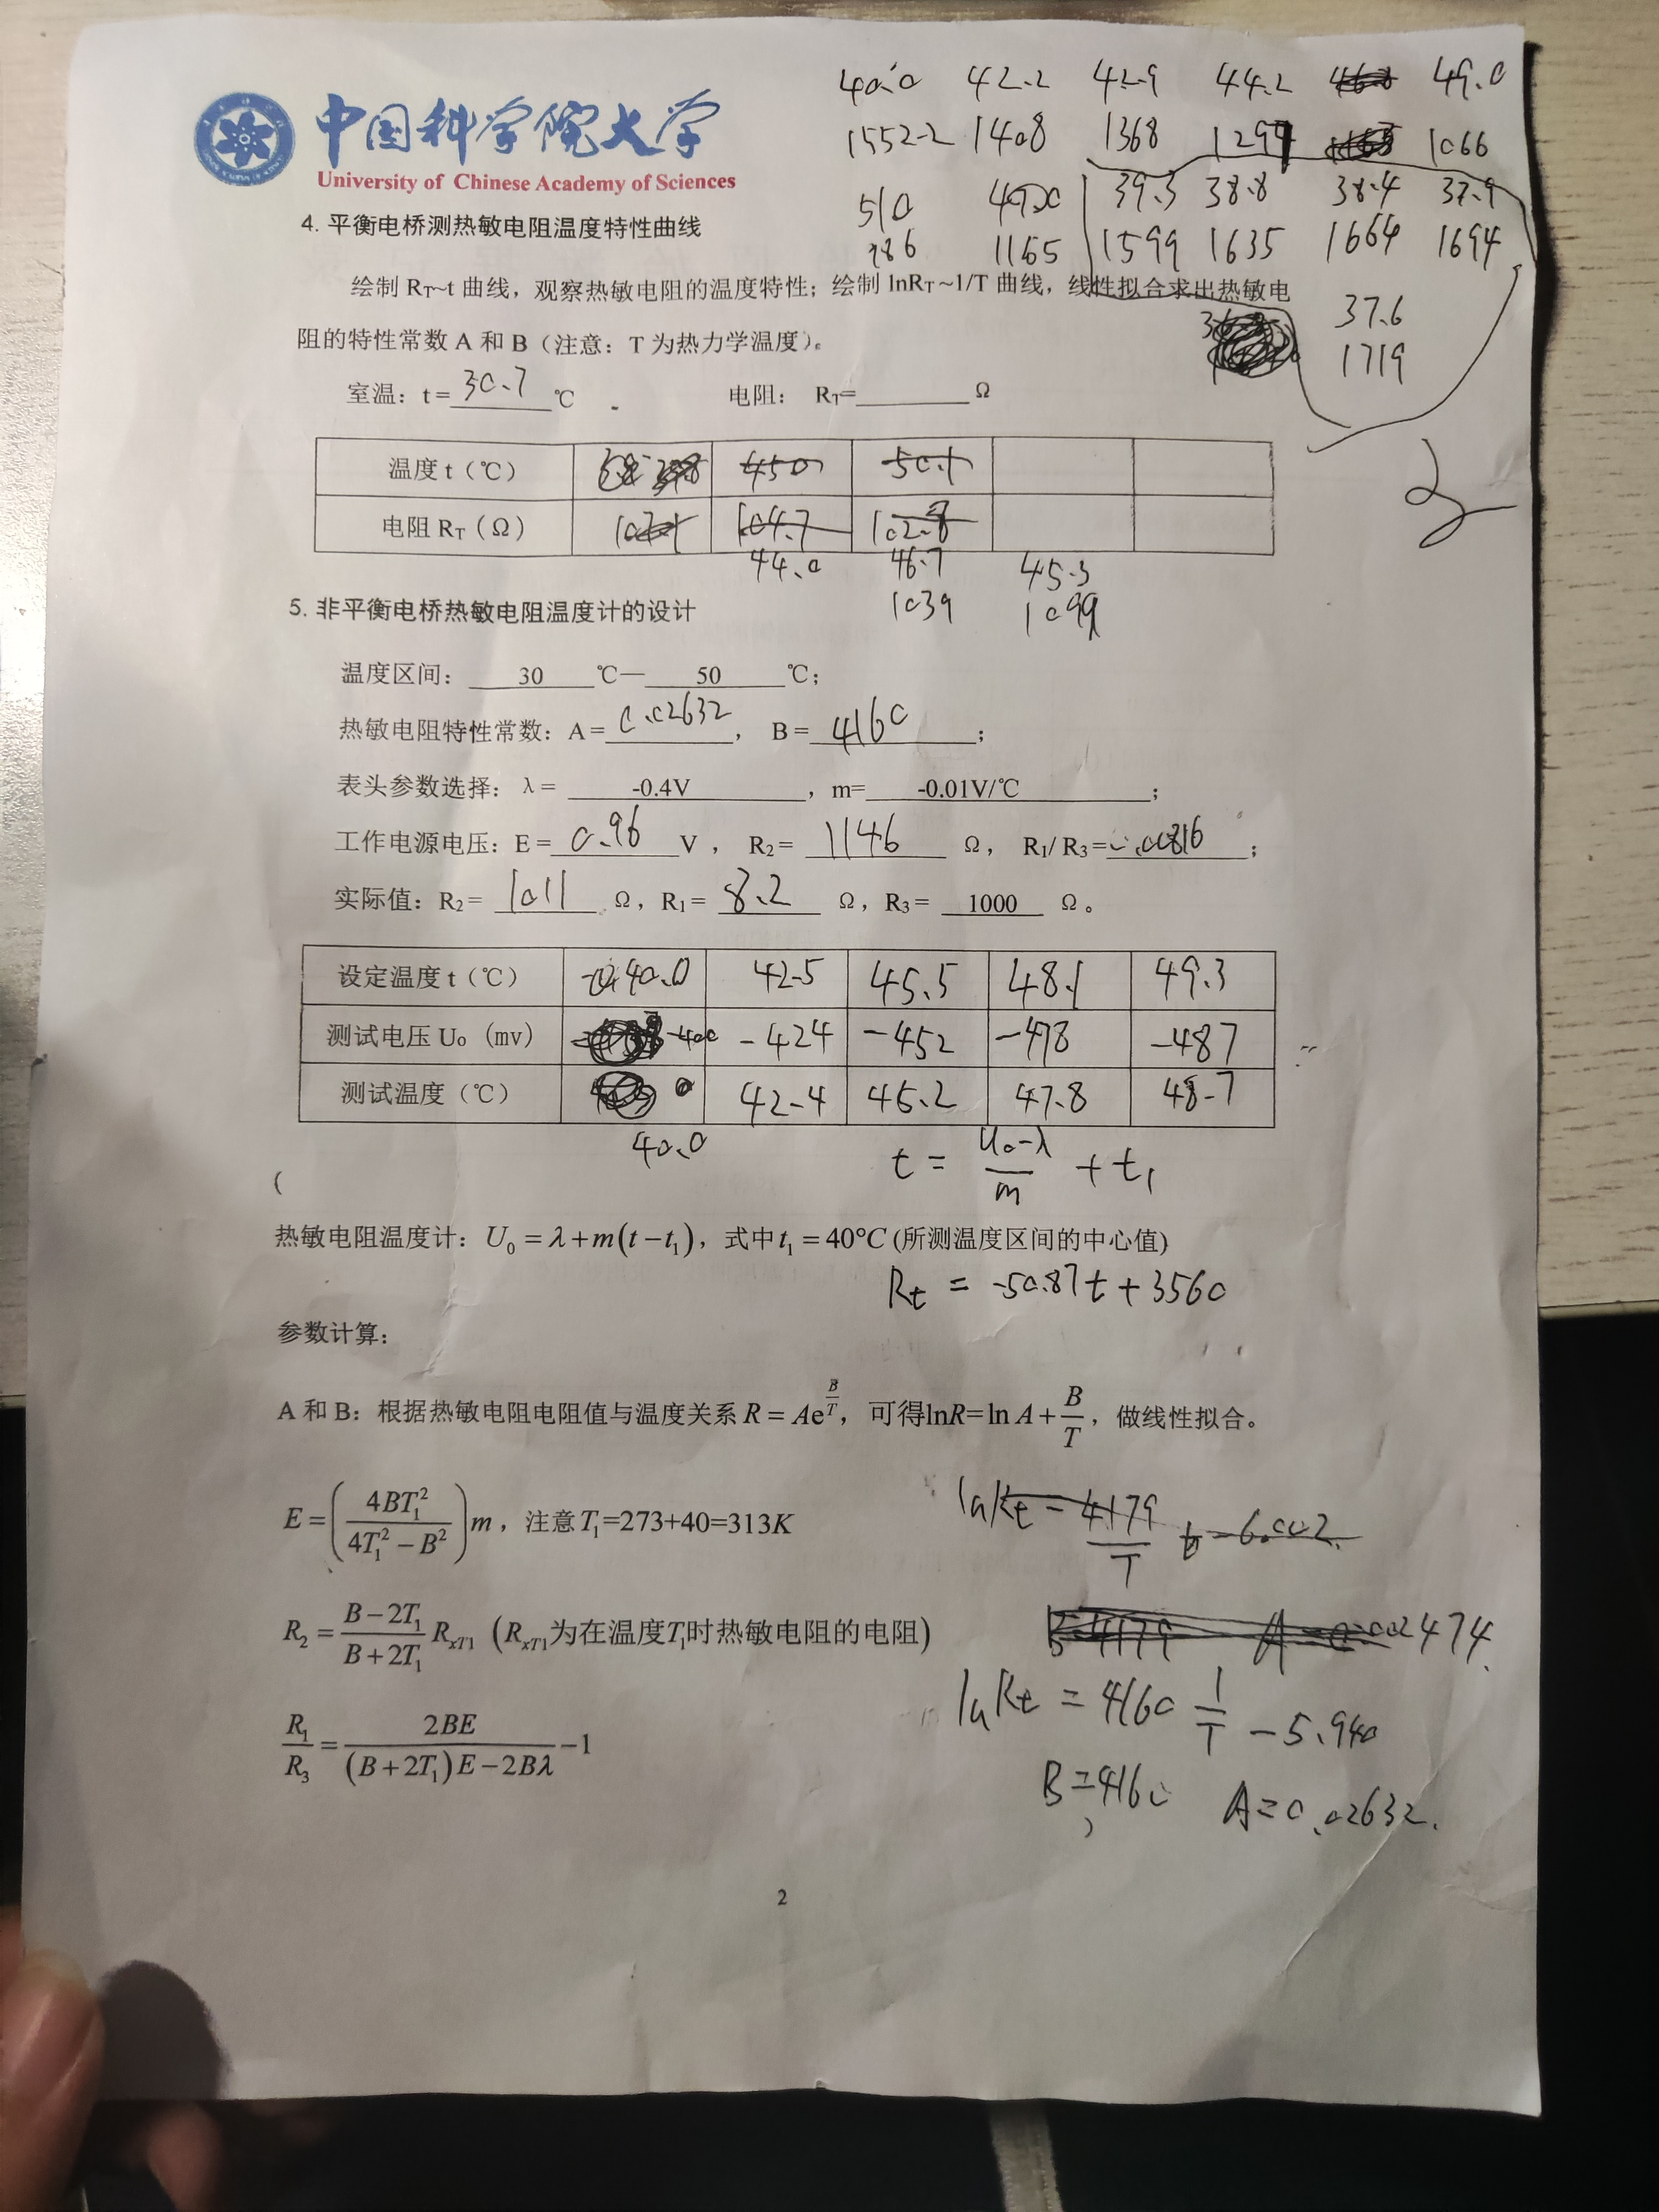
\includegraphics[width=15cm]{Fig/5.jpg}
        \caption{实验原始记录2}
    \end{figure}
    \begin{center}
        \vspace*{1em}
        \Large \bf 第四部分\qquad 预习报告
    \end{center}
    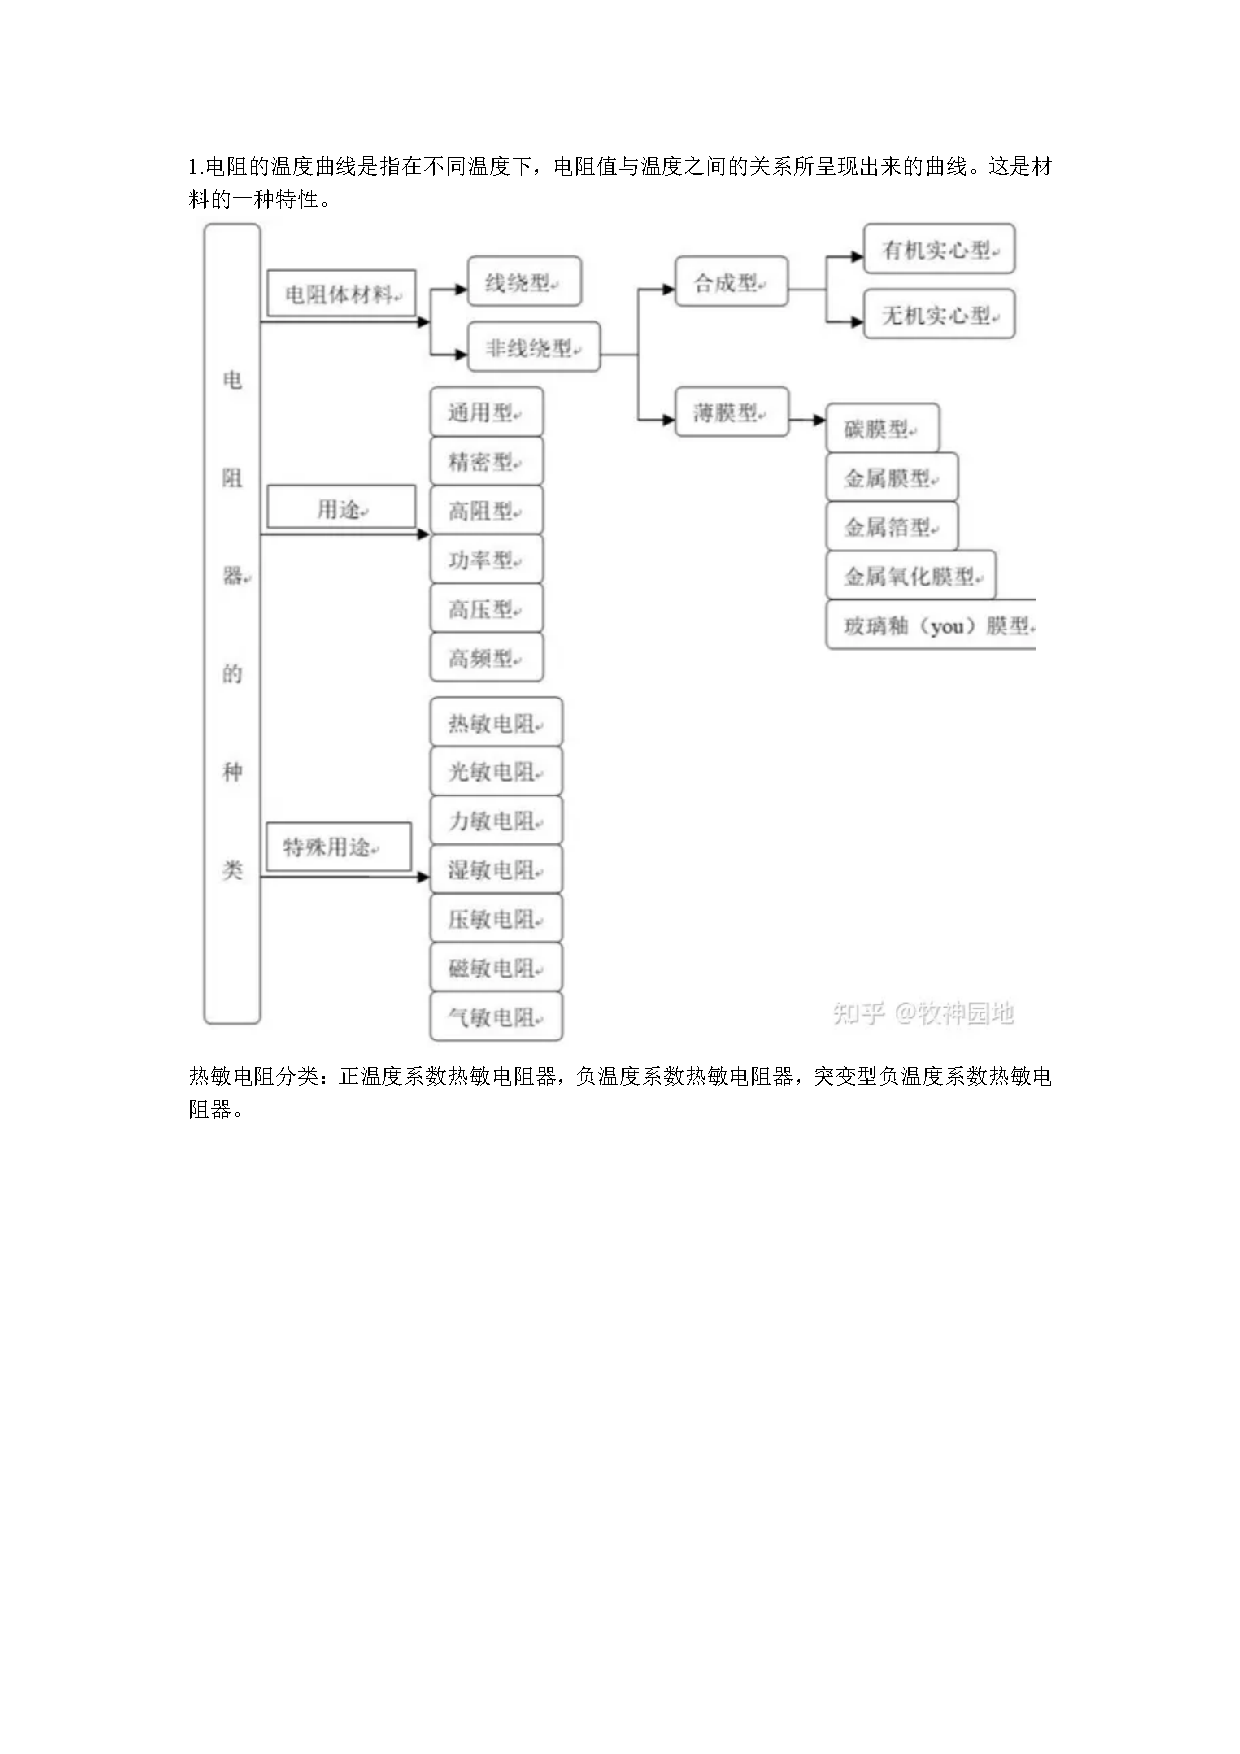
\includepdf[pages={1-3}]{预习报告.pdf}
\end{document}